\documentclass[11pt, a4paper]{article}
\usepackage[utf8]{inputenc}
\usepackage[T1]{fontenc}
\usepackage{polski}
\usepackage{graphicx}
\usepackage{float}
\usepackage{caption}
\usepackage{amsthm}
\usepackage{geometry}
\usepackage{longtable}
\usepackage{listings}
\usepackage{color}
\usepackage{subcaption}
\usepackage[section]{placeins}
\usepackage{fancyhdr}
\usepackage{graphicx}

\definecolor{dkgreen}{rgb}{0,0.6,0}
\definecolor{gray}{rgb}{0.5,0.5,0.5}
\definecolor{mauve}{rgb}{0.58,0,0.82}

\lstset{
  language=Java,
  aboveskip=3mm,
  belowskip=3mm,
  showstringspaces=false,
  columns=flexible,
  basicstyle={\small\ttfamily},
  numbers=none,
  numberstyle=\tiny\color{gray},
  keywordstyle=\color{blue},
  commentstyle=\color{dkgreen},
  stringstyle=\color{mauve},
  breaklines=true,
  breakatwhitespace=true,
  tabsize=3
}
\lstset{
  literate={ą}{{\k a}}1
  		     {Ą}{{\k A}}1
           {ż}{{\. z}}1
           {Ż}{{\. Z}}1
           {ź}{{\' z}}1
           {Ź}{{\' Z}}1
           {ć}{{\' c}}1
           {Ć}{{\' C}}1
           {ę}{{\k e}}1
           {Ę}{{\k E}}1
           {ó}{{\' o}}1
           {Ó}{{\' O}}1
           {ń}{{\' n}}1
           {Ń}{{\' N}}1
           {ś}{{\' s}}1
           {Ś}{{\' S}}1
           {ł}{{\l}}1
           {Ł}{{\L}}1
}

\geometry{
	a4paper,
	total={170mm,257mm},
	left=20mm,
	top=20mm,
}

\fancyhf{}
\fancyhead[L]{
\includegraphics[height=5.0mm]{PW.png}}

\fancyfoot{}
\renewcommand{\footrulewidth}{0.4pt}
\fancyfoot[C]{\thepage}

\setlength{\headheight}{6.50mm}
\pagestyle{fancy}

\title{\textbf{Uber Heals - specyfikacja implementacyjna}\\
    Algorytmy i struktury danych}
\author{Paweł Cegielski, Piotr Szumański, Jakub Matłacz}
\date{data utworzenia: 3 grudnia 2020\\
    data ostatniej zmiany: 14 grudnia 2020}

\usepackage{natbib}
\usepackage{graphicx}

\begin{document}

\maketitle

\section{Wstęp}
Program udostępnia mapę obiektów, szpitali oraz dróg pomiędzy nimi. Pozwala wczytać listę pacjentów pliku lub przy pomocy interfejsu graficznego. Wizualizuje transport tychże osób do najbliższych niepełnych szpitali.

\section{Opis ogólny}
    \subsection{Nazwa programu}
    Nazwa programu to Uber Heals.
    \subsection{Poruszany problem}
    Problemem jest optymalna dystrybucja pacjentów, jednocześnie przestrzegając nałożonych ograniczeń takich jak istnienie dróg między lokacjami, ilość wolnych łóżek w szpitalach oraz położenie najbliższego szpitala od lokacji pacjenta.
    \subsection{Użytkownik docelowy}
    Program stworzono dla pracowników służby ochrony zdrowia odpowiedzialnych za transport pacjentów.
    
\section{Opis implementacji}
    \subsection{Użyta technologia}
 Program zrealizowano przy użyciu języka programowania Java w wersji 13 w paradygmacie programowania obiektowego. Aby go uruchomić należy posiadać zainstalowane Java Runtime Environment (JRE w wersji 8) oraz bibliotekę JUnit 4 i JavaFX do realizacji GUI.
 
 \subsection{Struktura programu}
Program podzielono na klasy odpowiednialne za poszczególne zadania. Ponieżej (Rysunek 1) przedsta-wiono je wraz z ważniejszymi polami i metodami oraz asocjacje między nimi.
    \subsection{Sposób uruchamiania}
Należy uruchomić plik .jar i zaczekać na pokazanie się okna interfejsu graficznego. 
\subsection{Struktury danych}
W programie zastosowano ArrayList do przechowywania obiektów własnych klas oraz tablice, gdy potrzeba było większej szybkości.
\begin{figure}[ht]
    \centering
    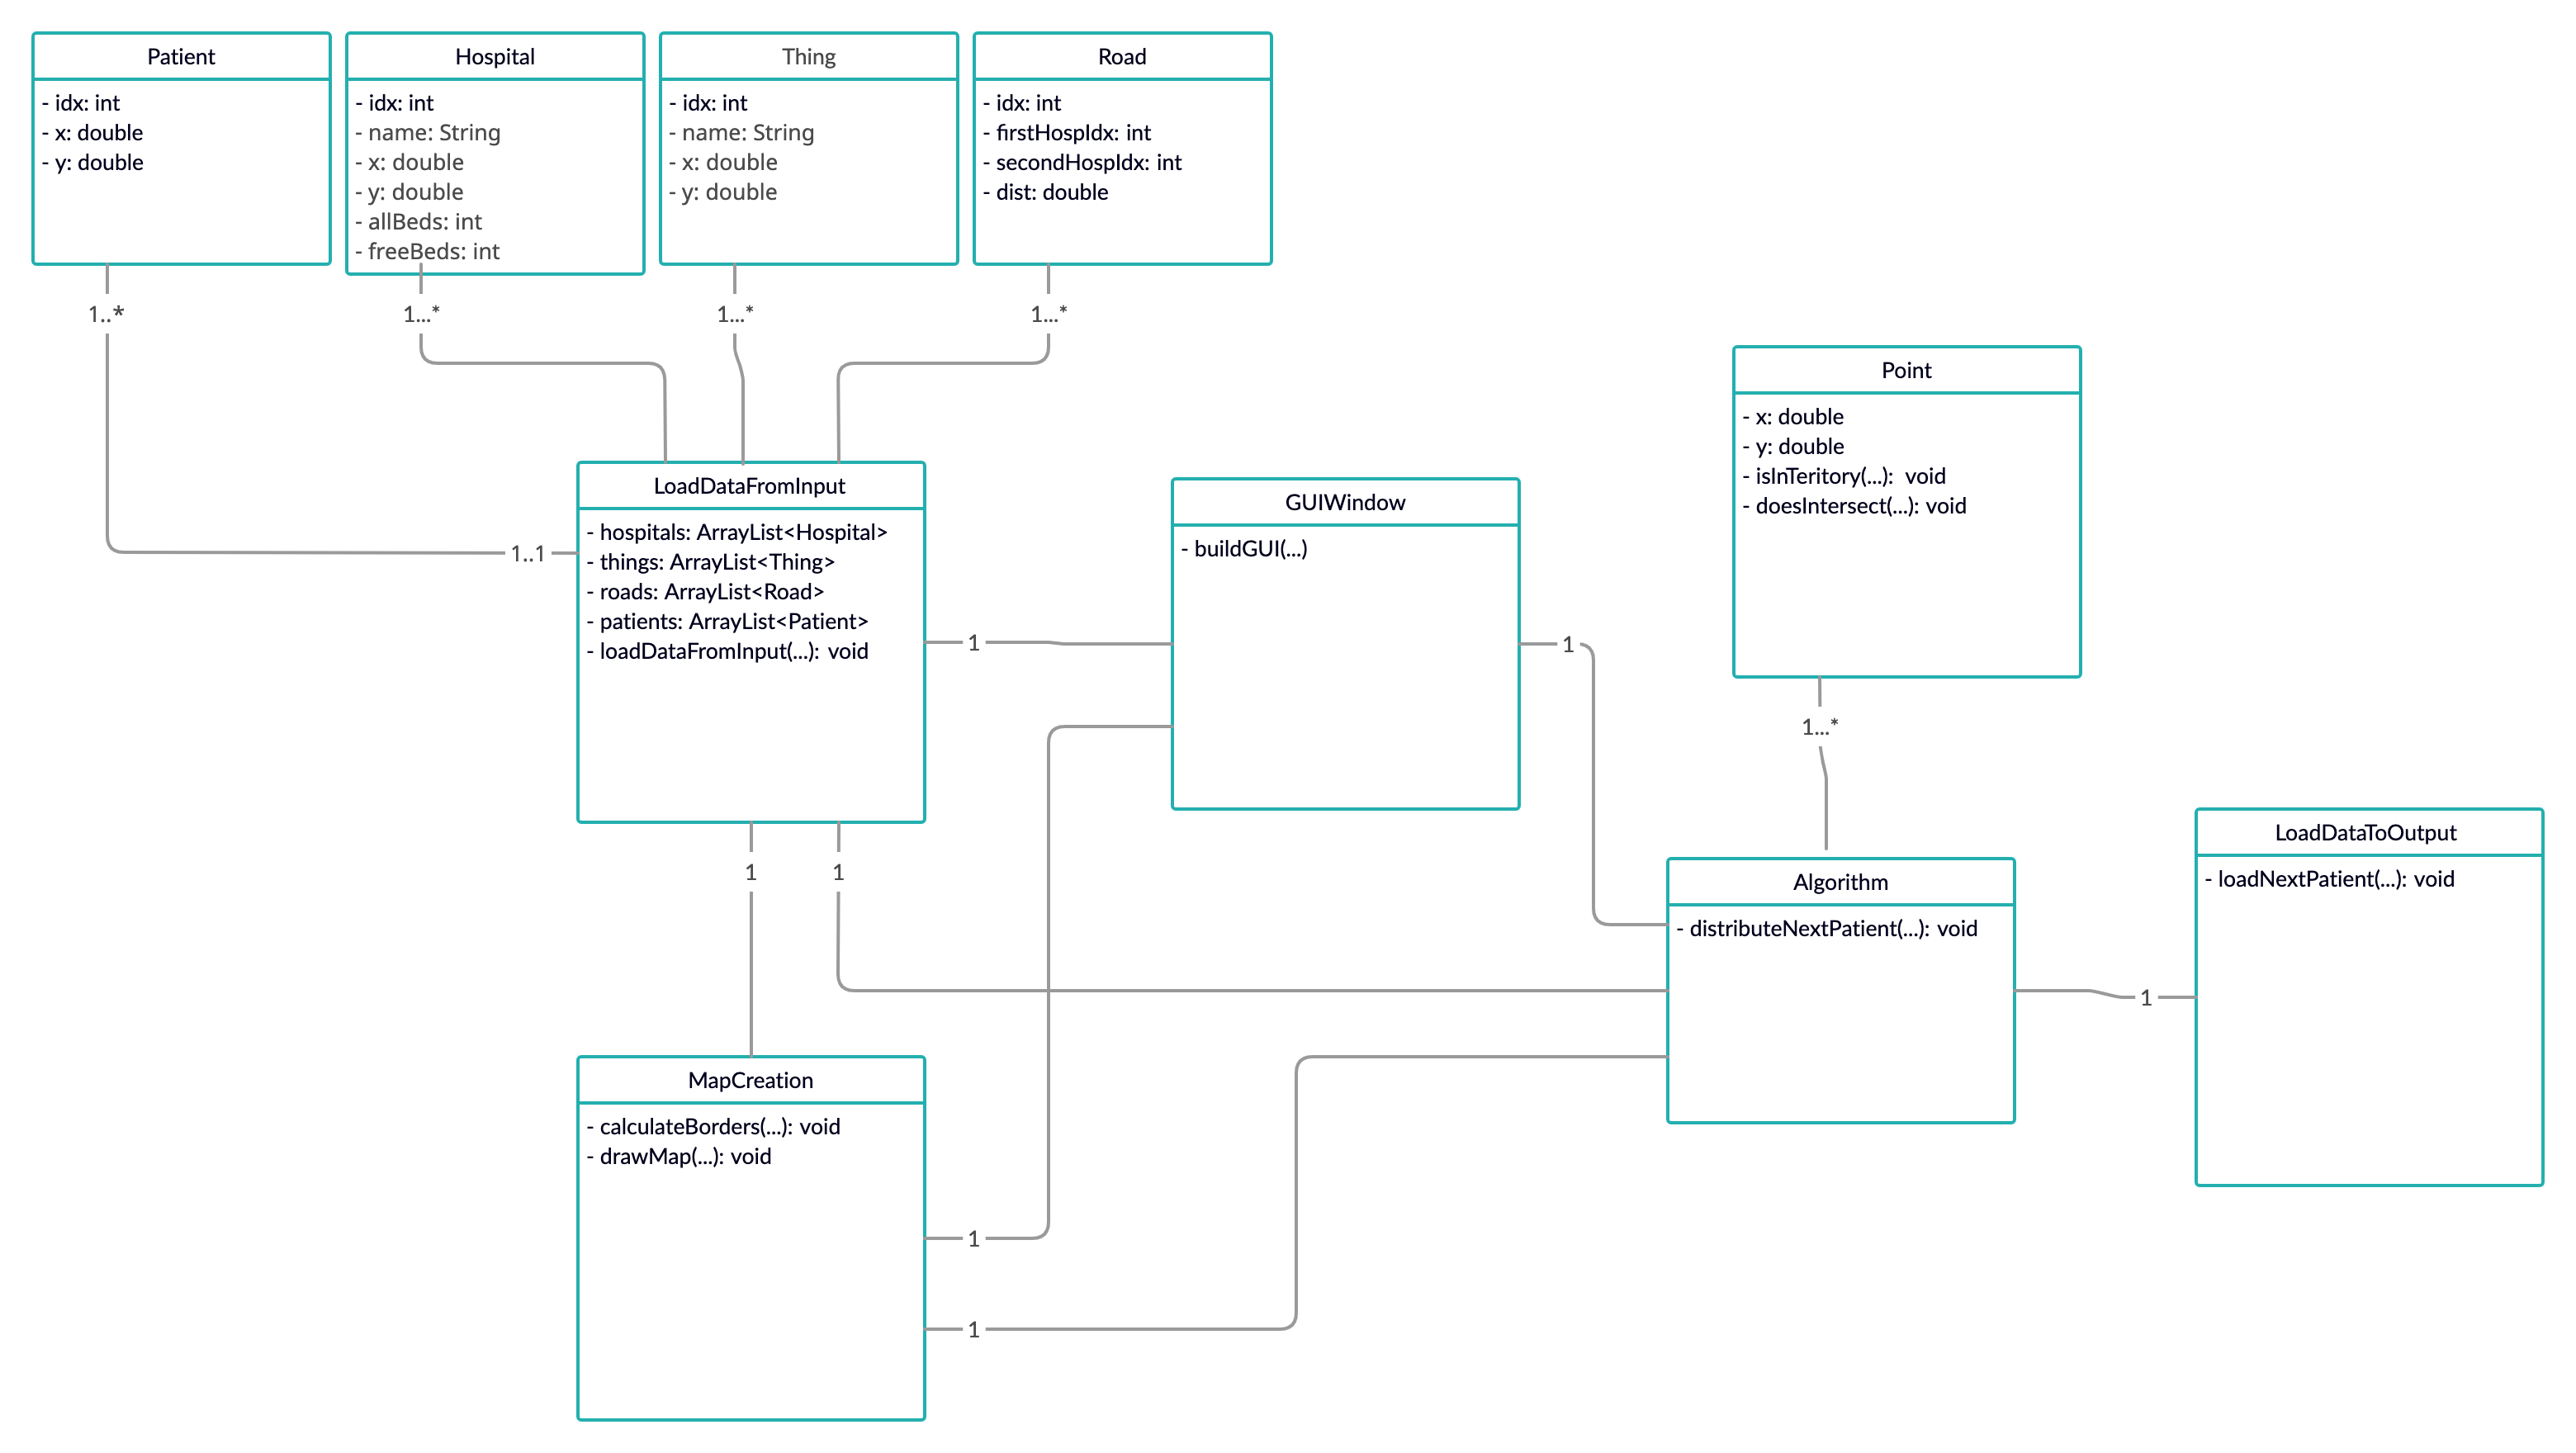
\includegraphics[width=1\textwidth]{diagramy.jpg}
    \caption{Diagramy klas}
    \label{fig:folder}
\end{figure}

    \subsection{Struktura katalogów}
    Taka jak na Rysunku 2.
    
    \begin{figure}[ht]
    \centering
    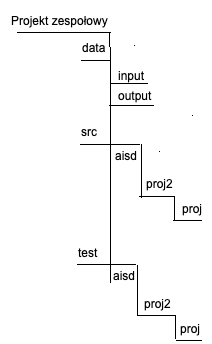
\includegraphics[width=0.3\textwidth]{katalogi.png}
    \caption{Struktura katalogów}
    \label{fig:folder}
\end{figure}

    \subsection{Wczytywanie pliku wejściowego}
Jeden z dwóch możliwych plików wejściowych można wczytać za pomocą obiektu klasy LoadDataFromInput z właściwym parametrem trybu (tryb wczytywania mapy lub pacjentów) oraz nazwą odpowiedniego pliku.

\begin{itemize}
    \item Sprawdzenie czy nazwa pliku jest właściwa
    \begin{itemize}
        \item Znaki alfanumeryczne
        \item Spacje, podłogi, myślniki
        \item Duże i małe znaki
        \item Rozszerzenie .txt
        \item Brak znaku potoku, pustej nazwy "", nazwy będącej samym ".txt", innego rozszerzenia
    \end{itemize}
    \item Sprawdzenie formatu pliku wejściowego
    \begin{itemize}
        \item Właściwy format wierszy danych
        \item Właściwy format nagłowków
        \item Posiadanie wszystkich nagłowków
        \item Oddzielanie wartości znakiem potoku
    \end{itemize}
    
    \item Wczytanie danych do pól klasy we właściwej formie
    \item Sprawdzenie spójności danych wejściowych
    \begin{itemize}
        \item Powtarzające się nazwy szpitali i obiektów
        \item Powtarzające się id szpitali, obiektów, dróg i pacjentów
        \item Powtarzające się pary id szpitali w drogach
    \end{itemize}
    \item Normalizacja identyfiaktorów dla dalszych obliczeń
    \item Przykładowy format plików wejściowych

    \begin{itemize}
    \item Plik mapy
    \begin{lstlisting}
# Szpitale (id | nazwa | wsp. x | wsp. y | Liczba łóżek | Liczba wolnych łóżek)
1 | Szpital Wojewódzki nr 997 | 10 | 10 | 1000 | 100
2 | Krakowski Szpital Kliniczny | 100 | 120 | 999 | 99
3 | Pierwszy Szpital im. Prezesa RP | 120 | 130 | 99 | 0
4 | Drugi Szpital im. Naczelnika RP | 10 | 140 | 70 | 1
5 | Trzeci Szpital im. Króla RP | 140 | 10 | 996 | 0

# Obiekty (id | nazwa | wsp. x | wsp. y)
1 | Pomnik Wikipedii | -1 | 50
2 | Pomnik Fryderyka Chopina | 110 | 55
3 | Pomnik Anonimowego Przechodnia | 40 | 70

# Drogi (id | id_szpitala | id_szpitala | odległość)
1 | 1 | 2 | 700
2 | 1 | 4 | 550
3 | 1 | 5 | 800
4 | 2 | 3 | 300
5 | 2 | 4 | 550
6 | 3 | 5 | 600
7 | 4 | 5 | 750
    \end{lstlisting}
    
    \item Plik pacjentów
    \begin{lstlisting}
# Pacjenci (id | wsp. x | wsp.y)
1 | 20 | 20
2 | 99 | 105
3 | 23 | 40
    \end{lstlisting}
    \end{itemize}

\end{itemize}



\subsection{Obliczanie dystrubucji pacjentów}
Dla każdego następnego wczytanego pacjenta otwieramy pętlę while, której warunkiem stopu jest przydzielenie pacjenta do szpitala lub informacja o tym, że wszystkie szpitale są już pełne. 
\begin{enumerate}
    \item Wczytanie pacjenta.
    \item Określenie czy należy do kraju, jeśli nie - koniec, przechodzimy do następnego pacjenta.
    \item Przeniesienie do najbliższego, pod względem odległości euklidesowej, szpitala.
    \item Przenoszenie pacjenta do kolejnego najbliższego (pod względem czasu podróży) szpitala tak długo, póki nie znajdzie się dla niego miejsce lub odwiedzi wszystkie możliwe szpitale i będą one pełne.
    \item Jeśli pacjent zostanie przyjęty przez szpital to należy zmniejszyć ilość wolnych łóżek.
\end{enumerate}

\subsection{Tworzenie pliku wyjściowego}
Plikiem wyjściowym naszego programu jest plik z logami, opisujący sekwencję zdarzeń - co dokładnie działo się z każdym pacjentem w kolejności.
W logach przedstawiamy dla każdego pacjenta dokładną trasę jaką przebył. Widać z jakich do jakich współrzędnych się przemieścił oraz ile czasu to zajęło (liczba w strzałce). Pokazano również nazwę szpitala wraz z ilością wolnych łóżek przed oraz po ewentualnym przyjęciu pacjenta.

\begin{itemize}
    \item Przykładowy format pliku wyjściowego
    \begin{lstlisting}
pacjent 0 :
(10,30) -10-> (5,10) szpital A 100/100 -> 100/100
(5,10) -5-> (10,20) szpital B 30/30 -> 30/30
(10,20) -20-> (30,40) szpital D 10/50 -> 11/50

pacjent 1 :
(12,50) -20-> (6,20) szpital E 120/120 -> 120/120
(6,20) -15-> (13,21) szpital F 25/30 -> 26/30
\end{lstlisting}
\end{itemize}

    

\section{Testy}
Program testowano w odrębych klasach testowych JUnit 4. Przyglądano się działaniu wyrażeń regularnych, poszczególnym metodom pomocniczym. Program testowano także jako całość podając różnepliki wejściowe (o różnych danych, rozmiarach, charakterystycznych cechach, szczególne przypadki)i sprawdzając pliki wyjściowe. Ponadto w tracie wykonywania programu na konsoli wyświetlane sąinformacje o zawartości struktur danych w poszczególnych iteracjach działania algorytmu. Stanowito proste logi programu, przydatne w procesie produkcji kodu oraz dla bardziej sprawnych przyszłych użytkowników. Wskazuje także na to czy program działa i ile iteracji potrzebuje na wykonanie zadania.
\subsection{Test całościowy systemu}
Ładowano pliki wejściowe podlegające testowaniu i sprawdzano w logach czy wykonywanie programu się kończy, w ilu iteracjach nastąpiło (efektywność).
\section{Podsumowanie}
Program został zaprojektowany tak, aby użytkownik mógł łatwo z niego korzystać podając plik mapy oraz plik pacjentów lub ręcznie podając pacjentów po kolei wraz z ich współrzędnymi. GUI pozwoli na wygodną i swobodną pracę z programem.
\end{document}
